\documentclass[border=0.2cm, convert={density=600}]{standalone}
 
% Required packages and libraries
\usepackage{tikz}
\usetikzlibrary{matrix, positioning, arrows.meta}

\tikzset{
	arrow/.style={
		draw=black,
		very thick,
		->,
		>=stealth
    },
}
 
\begin{document}
 
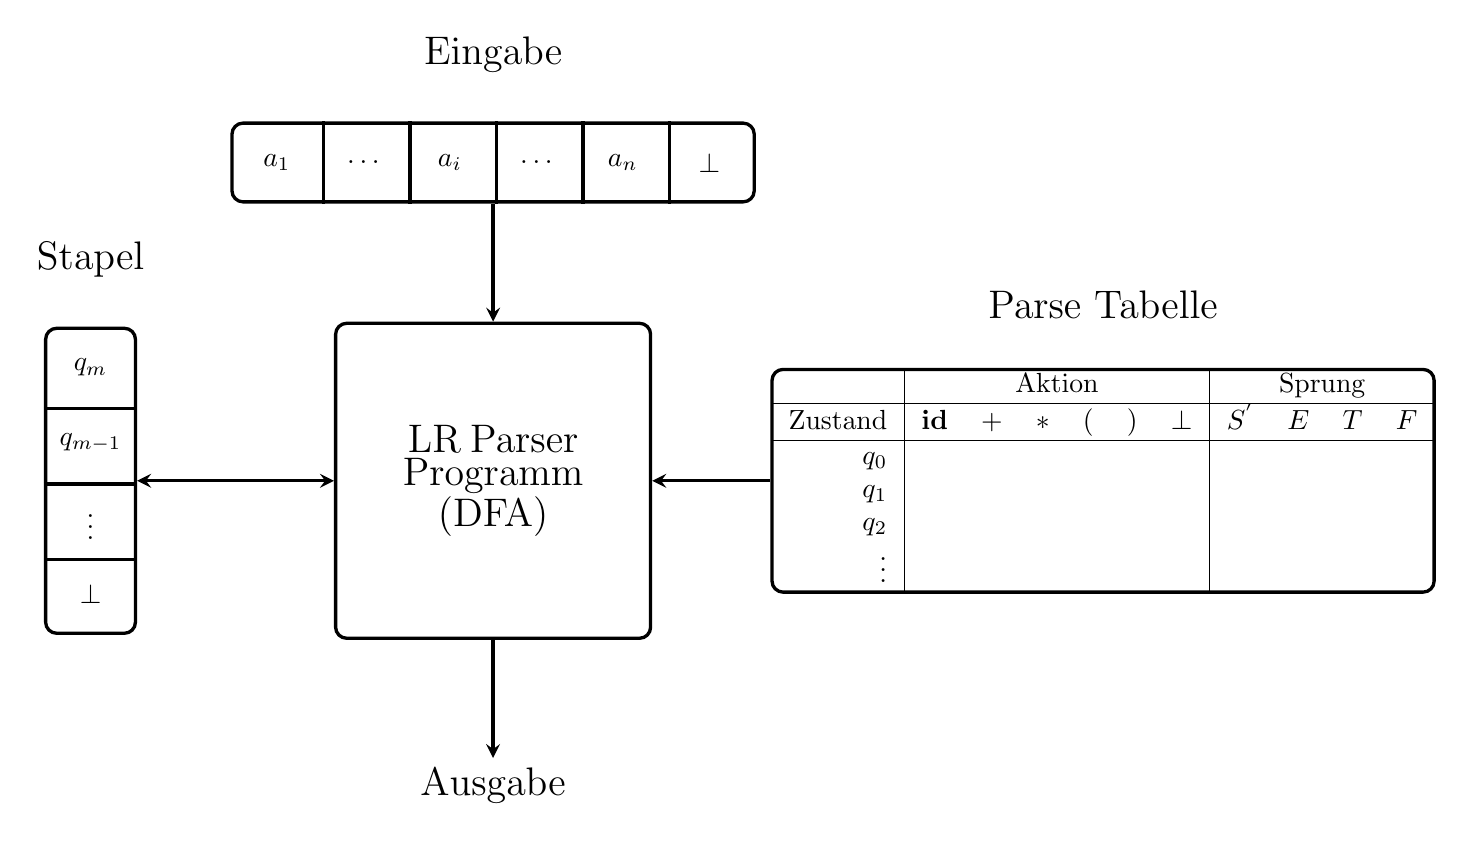
\begin{tikzpicture}

% Parsing Program
\node[
	draw=black,
	rectangle,
	very thick,
	rounded corners,
	text centered,
	text width=3cm,
	minimum height=4cm,
	minimum width=4cm,
	align=center,
	text=black,
	%anchor=center
] (Prog) {\Large LR Parser Programm (DFA)};

% Input
\matrix[draw,inner sep=0pt,very thick,rounded corners,above = 1.5cm of Prog] (In) [
	matrix of math nodes,
	column sep=-\pgflinewidth,
	row sep=-\pgflinewidth,
    nodes={text width=1cm,minimum height=1cm,align=center,text=black,anchor=center,sharp corners,inner sep=2pt}
] {
	a_1 & \ldots & a_i & \ldots & a_n & \bot\\ 
};
\draw[very thick] (In-1-1.north east) --(In-1-1.south east);
\draw[very thick] (In-1-2.north east) --(In-1-2.south east);
\draw[very thick] (In-1-3.north east) --(In-1-3.south east);
\draw[very thick] (In-1-4.north east) --(In-1-4.south east);
\draw[very thick] (In-1-5.north east) --(In-1-5.south east);

\node[above = 0.5cm of In] (InL) {\Large Eingabe};

% Parse Table
\node[draw,inner sep=0pt,very thick,rounded corners,right = 1.5cm of Prog] (Tab) {
\begin{tabular}{r|cccccc|cccc}
	& \multicolumn{6}{c|}{Aktion} & \multicolumn{4}{c}{Sprung}\\
	\hline
	Zustand & $\textbf{id}$ & $+$ & $\ast$ & $($ & $)$ & $\bot$ & $S^{'}$ & $E$ & $T$ & $F$\\
	\hline
	$q_0$   &               &     &        &     &     &        &         &     &     &    \\
	$q_1$   &               &     &        &     &     &        &         &     &     &    \\
	$q_2$   &               &     &        &     &     &        &         &     &     &    \\
	$\vdots$&               &     &        &     &     &        &         &     &     &    \\
\end{tabular}
};
\node[above = 0.5cm of Tab] (TabL) {\Large Parse Tabelle};

% Output
\node[below = 1.5cm of Prog] (Out) {\Large Ausgabe};

% Stack
\matrix[draw,inner sep=0pt,very thick,rounded corners,left = 2.5cm of Prog] (Stack) [
	matrix of math nodes,
	column sep=-\pgflinewidth,
	row sep=-\pgflinewidth,
    nodes={text width=1cm,minimum height=1cm,align=center,text=black,anchor=center,sharp corners,inner sep=2pt}
] {
	q_m\\
	q_{m-1}\\
	\vdots\\
	\bot\\
};
\draw[very thick] (Stack-1-1.south west) --(Stack-1-1.south east);
\draw[very thick] (Stack-2-1.south west) --(Stack-2-1.south east);
\draw[very thick] (Stack-3-1.south west) --(Stack-3-1.south east);

\node[above = 0.5cm of Stack] (StackL) {\Large Stapel};

% Arrows
\draw [arrow] (Prog) -- (Out);
\draw [arrow] (In) -- (Prog);
\draw [arrow,<->] (Prog) -- (Stack);
\draw [arrow] (Tab) -- (Prog);

\end{tikzpicture}
 
\end{document}

